\documentclass[10pt,a4paper]{article}
\usepackage[utf8]{inputenc}
\usepackage{amsmath}
\usepackage{amsfonts}
\usepackage{amssymb}
\usepackage{hyperref}

\usepackage{graphicx} % need this package



\begin{document}

\begin{titlepage}
    \begin{center}
        \vspace*{1cm}
        
        \Huge
        \textbf{Search Summary}
        
        
        \vspace{1.5cm}
        
        Author:
        \textbf{Nicolò Brandizzi}\\
        \vspace{0.5cm}
        \Large
        Contributors:
        \textbf{}%add contributors here
        
        \vfill
        
        
\includegraphics[width=0.4\textwidth]{images/sapienza_logo.jpg}


        
        \vfill
        
  

        \vspace{0.8cm}
        
        
        \Large
        DIAG\\
        Sapienza\\
        October 2018

    \end{center}
\end{titlepage}


\tableofcontents
\newpage
\begin{abstract}
This is \textbf{free} material! You should not spend money on it.\\
Find the complete material on GitHub \url{https://github.com/nicofirst1/AI_notes}.

This notes are about the \textit{Search} part taught by professor Daniele Nardi in the Artificial Intelligence class. Everyone is welcome to contribute to this notes in any relevant form, just ask for a pull request and be patient.\\ Remember to add your name under the contributors list in the title page when submitting some changes (if you feel like it).
\end{abstract}
\newpage


\section{Intro}

Some stuff you should remember:
\begin{itemize}
\item \textbf{Completeness}: The algorithm is guaranteed to find a solution when there is one.
\item \textbf{Optimality}: The strategy found is optimal.
\item \textbf{Time Complexity}: The time spent to find a solution
\item \textbf{Space Complexity} : The memory needed to perform the search.
\item \textbf{Branching factor} [b]: the maximum number of successors of any node.
\item \textbf{Depth} [d]: the depth of the shallowest goal node.
\item \textbf{[m]} : The maximum length of any path in the state space.
\end{itemize}



\newpage

\section{Uninformed Search}
Only use information available in the problem definition.

\paragraph{Breadth-first}
It expands the root node first and then all it's successors, and then it's successor and so on. It can be implemented using a \textit{FIFO} queue where the goal condition is applied to each node when it is \textbf{generated}.\\
Proprieties:
\begin{itemize}
\item Complete if $d<\infty$ 
\item Optimal if the path cost is a non-decreasing function of the depth (all action have same cost)
\item Time and Memory complexities are $O(b^{d+1})$
\end{itemize}

\paragraph{Uniform-cost}
Expands the node with the lowest path cost [$g(n)$]. It can be implemented using a \textbf{Priority Queue} ordered by $g(n)$. The goal condition is applied to the node when this one is selected for \textit{expansion} because the generated one can be a sub-optimal path.\\
Proprieties:
\begin{itemize}
\item Complete if $g(n)>\epsilon$
\item Always Optimal  since it expands the nodes in order of their optimal path cost
\item Time and Memory complexities are $O(b^{C*/\epsilon})$, where $C*$ is the cost of the optimal solution
\end{itemize}

\paragraph{Depth-first}
Expands the deepest node in the frontier, using a \textsc{LIFO} queue.
\begin{itemize}
\item Complete for \textit{graph version} if space is finite, not complete for \textit{tree version}
\item Not Optimal
\item Time Complexity is $O(b^m)$ where $m$ is the maximum depth of any node
\item Space Complexity is $O(b\cdot m)$ 
\end{itemize}


\paragraph{Depth-limited}
Is the same as \textit{depth-first} but there is a limit for the maximum depth $l$.

\begin{itemize}
\item Complete for $l \ge d$
\item Optimal for $l \le d$
\item Time Complexity is $O(b^l)$ 
\item Space Complexity is $O(b\cdot l)$ 
\end{itemize}

\paragraph{Iterative deepening depth-first}
Same as \textit{Depth-limited} but gradually increases $l$ until we have $l=d$.

\begin{itemize}
\item Complete when path cost is non decreasing.
\item Space Complexity is $O(b\cdot d)$ 
\item Time Complexity is $O(b^d)$ 
\item Optimal if the path cost is a non-decreasing function of the depth (all action have same cost)

\end{itemize}

\paragraph{Search Direction}
Can be 
\begin{itemize}
\item \textbf{Forward}: or data driven
\item \textbf{Backward}: or goal driven 
\item \textbf{Bidirectional}:
Uses two simultaneous searches, one from start to goal and one from goal to start, hoping the searches will meet in the middle. It is less intensive since $b^{d/2}+b^{d/2}<<b^d$.
\end{itemize}



\newpage

\section{Informed Search}

Some algorithm make use of an evaluation function $[f(n)]$ to decide which node to expand first (lowest). This information can be joint with an heuristic function $[h(n)]$ which \textbf{estimate the cost of the cheapest path from the current state (node n) to the goal}.

\subsection{Heuristic functions}


\paragraph{Dominance}
A heuristic function $h_1(n)$ \textbf{dominate} another $h_2(n)$ if 
\[\forall n : h_1(n) \ge h_2(n)\]
This leads to the following propriety: \textbf{the number of nodes expanded by A* with a dominant h is always less}.

\paragraph{Admissibility}
For tree search the heuristic function needs to be \textbf{admissible}, that is the function never overestimate the cost to reach the goal. For example the path to get from Rome to Madrid being a straight line (euclidean distance) rather than following the roads and avoiding the sea will be an underestimation of the real path.

\paragraph{Consistency}
For graph search the heuristic function must be \textbf{consistence} \footnote{Every consistent heuristic is also admissible}, i.e. the estimate cost to reach the goal from n is not grater than the cost to reach the node $n'$ (child of n) plus the estimated cost from n' to the goal\footnote{Also known as triangle inequality}
\[h(n) \le c(n,n')+h(n')\]
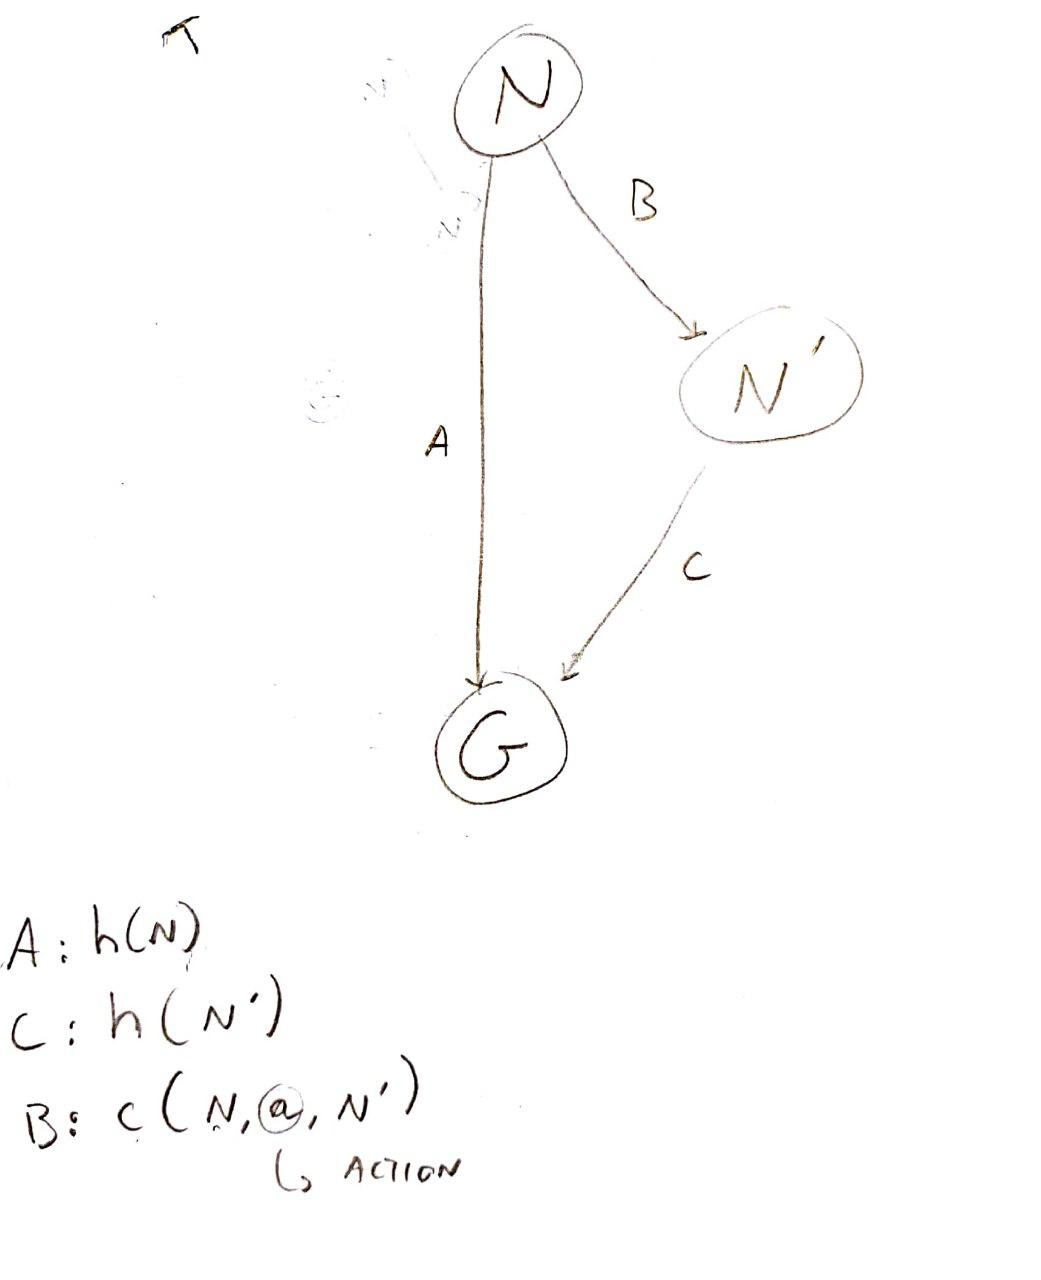
\includegraphics[scale=0.2]{images/consistency.jpg}


\paragraph{Relaxed problem}
The optimal solution of a relaxed problem is not grater than the optimal solution of the real one. So you can derive a heuristic function from the relaxed problem and apply it to the real one.

\paragraph{Combination}
Given multiple heuristics $h_1(n),h_2(n),...,h_m(n)$ you can combine them into a heuristic function which dominates all of them:
\[\forall n: h(n)=max(h_1(n),h_2(n),...,h_m(n))\]

\paragraph{Effective Brancing Factor [EBF]}
Given an algorithm whose looking for a goal node and two heuristics associated with it, $h_1(n),h_2(n)$. This algorithm expands $N_1=17$ nodes before reaching the solution with the first heuristic and $N_2=14$ with the second. Moreover the expansion tree has a brancing factor  \footnote{The number of successors generated by a given node.} of $d=3$. To measure the effectiveness of a heuristic we estimate the \textbf{effective brancing factor} [EBF]:
\[N+1=1+EBF+EBF^2+...+EBF^d\]
For our example we have:
\[17+1=1+EBF_1+EBF^2_1+EBF_1^3\rightarrow EBF_1\approx 2.165\] 
\[14+1=1+EBF_1+EBF^2_1+EBF_1^3\rightarrow EBF_1= 2\]
The closer EBF is to one the better the heuristic is.

\paragraph{Greedy best-first search}
This algorithm uses just the information from the heuristic function. The proprieties are the following:
\begin{itemize}
\item \textbf{Not complete}: can get stuck into loops, can be complete only in finite state with checking.
\item \textbf{Not Optimal}

\item \textbf{Time} $O(b^m)$ where $m$ is the maximum depth of the node and $b$ is the branching factor.
\item \textbf{Space} $O(b^m)$, keeps every node in memory.
\end{itemize}

\subsection{A*} 
If we combine the information given by the heuristic function, i.e. the cost to reach the goal from the current node, \textbf{h(n)} and the cost to reach the node \textbf{g(n)}, we get an \textbf{estimated cost of the cheapest solution through the node n}
\[f(n)=g(n)+h(n)\] 


\paragraph{Optimality of A*}
Proving that A* is optimal if h(n) is consistent is fairly easy, we just need to use the formulation of consistency:
\[f(n')=g(n')+h(n')=g(n')+c(n,n')+h(n') \ge g(n)+h(n)=f(n)\]\footnote{Guarantees that $f$ is not decreasing (monotonic).}
Moreover the sequence of nodes expanded by A* is in non-decreasing order, hence the first node must be an optimal solution because $f$ is the true cost for the starting point ($h(n_s)=0$)

\paragraph{Proprieties of A*}
\begin{itemize}
\item \textbf{Is complete} unless there are infinitely many nodes with $f \le f(G)$
\item \textbf{Is Optimal}

\item \textbf{Time is exponential}
\item \textbf{Space}, keeps every node in memory

\end{itemize}


\subsection{Other implementation of A*}
The A* algorithm has some limitations, the most important is the exponential use of the memory (we keep every node in memory).

\paragraph{Iterative Deepening A* [IDA*]}
The cutoff value is the value of $f(n)=g(n)+h(n)$ rather than the three depth. This behave well for unit cost path finding problems, and keeps a linear memory consumption. But has the same problem of the uniform-cost search

\paragraph{Recursive Best First Search [RBFS]} 
It goes down a node recusivley until the \textit{f-value} increases above the alternative nodes. When this happens it rewinds back to the original node storing the \textit{f-value} of its children. Each rewind and change of mind is an IDA* iteration.\\
Is has \textbf{O(bd)} complexity for space, but its time complexity is not easy to characterize, moreover it uses \textit{too few memory} (only the \textit{f-values} of nodes are stored) thus it can expand a path multiple times.

\paragraph{Simple Memory Bounded A* [SMA*]}
It behaves just like A*, but when its memory is full it drop worst leaf node \footnote{The one with the highest \textit{f-value}.} propagating its \textit{f-value} up to its parent. When there are same \textit{f-valued} nodes it always expand the newest and deletes the oldest. This algorithm is always complete if the depth (d) of the shallowest solution is in memory size reach.\\
Proprieties:
\begin{itemize}
\item Uses all available memory
\item It avoids to repeat states until the memory is full
\item It is complete and optimal if $d$ can fit in memory
\end{itemize}


\newpage

\section{Local Search Algorithms}

Sometimes we don't know the entirety of the state space or we just don't care of the path to reach the goal. For this kind of problem we adopt the local search algorithm whose objective is to gradually optimize a state.

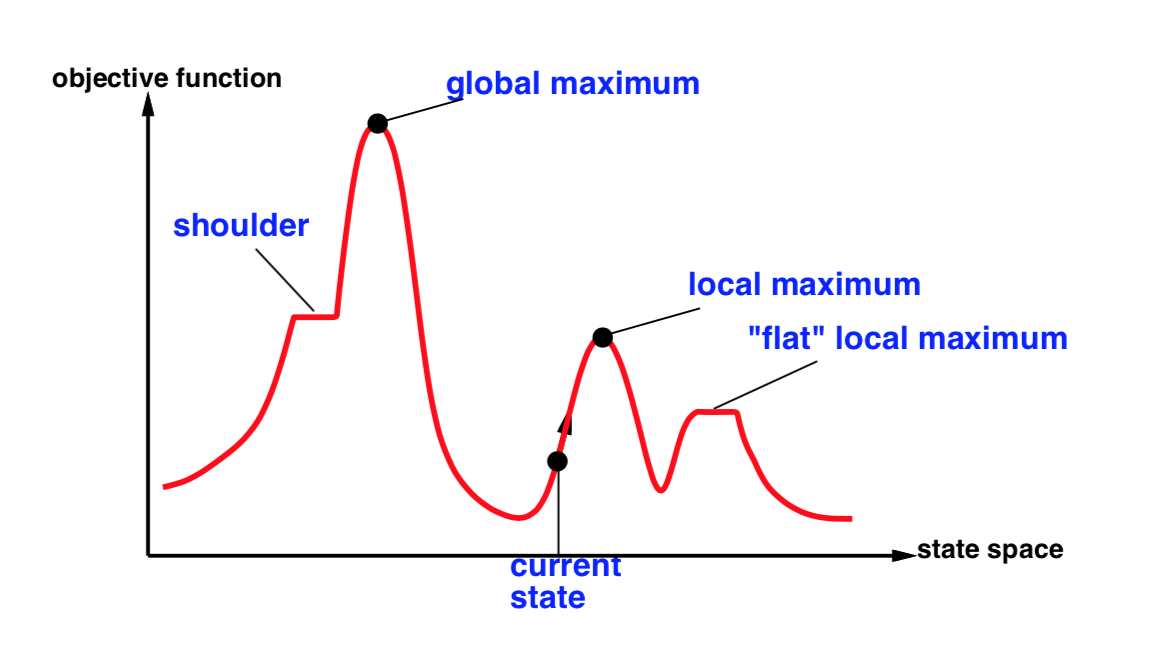
\includegraphics[scale=0.7]{images/problems.png}


\subsection{Hill-climbing search}
Hill climbing is a simple loop which moves in the direction of the increasing value \footnote{The value is given by an heuristic function.}. Since this algorithm is a \textbf{greedy local search} it grabs  a good neighborhood without thinking ahead, for this reason it can get stuck in the following cases:
\begin{itemize}
\item \textbf{Local Maxima}: it won't come down from the maximum (even if it's only local)
\item \textbf{Ridges} : are a sequence of local maxima which are difficult to navigate \footnote{Look it up on google.}.
\item \textbf{Plateaux} : a flat surface which can be either a local minimum or a shoulder.
\end{itemize}

\paragraph{Stochastic hill-climbing}
Chooses a randomly from the possible uphill moves, it is slower but can find better solutions.

\paragraph{First choice hill-climbing} 
Implements stochastic hill climbing by generating successors randomly until one is generated that is better than the current state

\paragraph{Random restart hill-climbing}
Randomly generates initial states until a goal is reached. If each hill-climbing has a probability $p$ of succeed then the expected number of restarts required will be $\frac{1}{p}$.


\subsection{Simulate annealing}
It is a midway between the hill-climbing algorithm and a randomize search \footnote{Moving to a successor chosen uniformly at random from the set of successors}. The algorithm picks a random moves every time, if the moves decreases the total cost then it is accepted, on the other hand it has a probability $p$ to be accepted. The probability $p$ depends on two factor:
\begin{itemize}
\item The \textbf{schedule T} which is a sort of time measure from the start of the algorithm, the more time has passed the lower $p$ will be
\item The \textbf{badness $\delta E$} of the choice to be accepted, i.e. how much worst is the cost after accepting the choice.
\end{itemize}

If the schedule is slow enough then the algorithm approaches probability 1 to reach a goal. 

\subsection{Beam Search}
This algorithm keeps track of $k$ random generated states, compares them with each other and picks the $k$ best from their successors. Useful information is passed between the $k$ threads so that unfruitful states are abandoned to prefer best ones.\\
 This can bring the search to be concentrated in a small region of the state space. To fix this there is another implementation called the \textbf{stochastic beam search} which chooses $k$ successors at random with a probability which is a function of the increasing value.
 
\subsection{Genetic Algorithm [GA]}
GAs combine uphill tendency with a random exploration of the state space and information exchange between parallel states. The algorithm works like this:
\begin{enumerate}
\item At first $k$ random states are generated, called the \textbf{population}.
\item The GA rate states using a \textbf{fitness function} which return a higher value for better states.
\item A pair of states are chosen according to the rating and a \textbf{crossover}\footnote{The crossover usually take large steps at the beginning of the algorithm } point is defined randomly from the states.
\item Finally a random mutation occurs in the children.
\end{enumerate}



\newpage

\section{Constraint Satisfaction Problems [CSP]}
A CSP has three elements:
\begin{itemize}
\item A set of \textbf{variables} ${X_1,X_2,...,X_n}$, which becomes states when $X_i$ takes its values from $D_i$.
\item A set of \textbf{domains} for each variable ${D_1,D_2,...,D_n}$
\item A set of \textbf{constrains} $C$ for legal variable combinations. Which is later called \textit{goal test}.
\end{itemize}



It is helpful to visualize a CSP as a constraint graph in which every node is a variable and the edges are the constrains. This is done in order to apply \textit{constraint propagation} and delete large portions of search space from the searching.

\subsection{Variations of CSP}
The simplest kind of CSP have a discrete finite domain. When the domain is not finite (although is discrete) we must use a constraint language to express the link between variables without enumerating all the legal combinations. \\
As long as the domain is discrete this types of CSP fall under the category of \textbf{linear programming} which can be solved in time polynomial to the number of variables.

\paragraph{Aryties constrains}
There are different kind of constrains:
\begin{itemize}
\item \textbf{Unary constrains} where a variable is bounded to be a single value ($X=1$), they can be treated as a domain restriction.
\item \textbf{Binary constrains} that relates two variables together ($X\neq Y$)
\item \textbf{Higher order constrains} like $Y\le X \le Z$, can be reduced increasing the number of variables and constraints.
\item \textbf{Global constrains} which involves an arbitrary \footnote{Not necessarily all the variables.} number of variables (like $AllDiff(X_1,X_2,..,X_n)$)
\end{itemize}

\paragraph{Constraint Optimization Problems [COP]}
Indicates which solution is preferred, this kind of constrains are not forcefully respected but rather are costly to be neglected.



\subsection{Inference in CSPs}
We can use \textbf{constraint propagation} to reduce the number of legal values for a variable.

\paragraph{Node consistency} 
A single variable is node-consistent if all the values in the variable's domain satisfy the variable's unary constraints. It is always possible to eliminate all the unary constraints in a CSP by running node consistency.

\paragraph{Arc consistency}
A variable in a CSP is arc-consistent if every value in its domain satisfies the variable’s binary constraints. 
For example given $Y=X^2$ with :
\[\langle(X,Y),[(0,0),(1,1),(2,4),(3,9)]\]
If we want to make $Y$ arc-consistent in respect to $X$ we remove from the Y's domain those value which cannot be taken from the equation, so the Y domain will become $[0,1,4,9]$.\\
The \textbf{Ac-3} algorithm is used to propagate arc-consistency in a CSP, it works like this:
\begin{enumerate}
\label{AC3}
\item Initially the queue contains all the arcs in the CSP.
\item AC-3 pops arbitrary arc $(X_i,X_j)$ from the queue.
\item It makes $X_i$ consistent with $X_j$
\item If this leaves $D_i$ unchanged it continues, else $D_i$ got smaller and the AC-3 gets all the arcs neighborhood of $X_i$ and adds them to the queue
\item If $D_i$ ends up empty the AC-3 return a failure
\item Else it returns the subset of the original domain.
\end{enumerate}

The algorithm lead to faster search at the cost of executing the AC-3 which is $O(cd^3)$ in the worst case scenario.

\paragraph{Path consistency}
Almost the same as the arc-consistency, in this case we look at a triple of variables $X_1,X_2,X_3$.
A two-variable set ${X_1,X_3}$ is path-consistent with respect to a third variable $X_2$ if, for every assignment ${X_1 = a, X_3 = b}$ consistent with the constraints on ${X_1 , X_3 }$, there is an assignment to $X_2$ that satisfies the constraints on ${X_1 , X_2 }$ and ${X_2 , X_3 }$. This is called path consistency because one can think of it as looking at a path from $X_1$ to $X_3$ with $X_2$ in the middle.

\paragraph{K-consistency}
A CSP is strongly k-consistent if it is k-consistent and is also \textit{(k-1)-consistent, (k-2)-consistent, \dots all the way down to 1-consistent}. Now suppose we have a CSP with n nodes and make it strongly n-consistent, for each $X_i$ we need to find the values in its domain which are consistent with $X_1,X_2,...,X_{i-1}$. We will find a solution in $O(n^2d)$ time using exponential space!

\paragraph{Global constrains}
\textbf{Resource constraints} (also called \textit{atmost} constraint), for example the constraint that no more than 10 personnel are assigned in total is written as $AtMost(10,P_1,P_2,P_3,P_4)$ and can be checked estimating the sum.\\
But for large resource-limited problems with integer value we use \textbf{bounds propagation}. For example:\\
$F_1$ and $F_2$ are to flights, for which the planes have capacities 165 and 385, respectively. The initial domains for the numbers of passengers on each flight are then:
\[D_1=[0,165] \quad \quad D_2=[0,385]\]
Now suppose we have the additional constraint that the two flights together must carry 420 people: $F_1+F_2=420$, propagating bounds constraints leads to :
\[D_1=[35,165] \quad \quad D_2=[255,365]\]

\subsection{Backtracking for CSP}

We know that CSPs are \textbf{commutative} since the assignment of a variable to a value reach the same partial assignment given any order \footnote{This brings the possible combination in Sudoku from $n!*d^n$ to $d^n$}. The \textit{backtracking search } is the same as a depth-search but when a leaf has no legal value left it backtrack the information to its root.

\paragraph{Values and variable order}
There are some ways to choose the order of variables/values to optimize the time spent building the three.
\begin{itemize}
\item \textbf{Minimum Remaining Value [MRV]} : choosing the variable with the fewest \textit{legal} values.
\item \textbf{Degree Heuristic} : it attempts to reduce the branching factor on future choices by  selecting the variable that is involved in the largest number of constrains.
\item \textbf{Least constraining value}: it prefers the value that rules out the fewest choices for the neighboring variables in the constraint graph.
\end{itemize}

\paragraph{Search and Inference}
There are some techniques to check whenever a choice is better than another. One of them is \textbf{forward checking} in which we chose a values for a variable $X_i=c$ and we remove $c$ from all the domains of the variables connected to $X_i$. This is the case of the constrain \textit{AllDiff}, but the technique works for other examples too.\\
Another one is \textbf{Maintaining Arc Consistency [MAC]}: when a value is decided for the variable $X_i$ the algorithm calls AC-3 [\ref{AC3}] to check arch consistency on all the variables connected with $X_i$.

\paragraph{Looking Backwards}
A problem that we may face is the choosing of the right variable $X_i$ which is in direct conflict with the considered variable $X_j$. There might be cases of an illegal assignment between this two variables but an arbitrary number of other variables $(Y_1,Y_2,...,Y_k)$ were chosen in the meanwhile. So the previous algorithm will just jump back from $X_j \rightarrow Y_K \rightarrow Y_{k-1} \rightarrow ...\rightarrow Y_1 \rightarrow X_i$ arriving at the actual problem after $k$ futile approaches. \textbf{Back-jumping} is used to store a \textbf{conflict set} of each variable so that, when an illegal assignment occurs, we can directly jump back to the cause of it.\\
Remember that every branch pruned by backjumping is also pruned by forward checking.



\end{document}




















